\FloatBarrier
\section{Studio di Caso ed Esercizi Analitici su DTW}
\label{sec:ts-dtw-exercises}

In questa sezione si risolve in modo rigoroso e formale un problema classico d'esame articolato in tre quesiti analitici.

\FloatBarrier
\subsection{Formulazione del Problema}
\label{subsec:ts-exercise-problem}

Siano assegnate le seguenti serie temporali di lunghezza $n=5$:
\begin{equation}
\label{eq:ex-input-series}
t_1 = \langle 4, 3, 6, 1, 0 \rangle, \quad t_2 = \langle 3, 6, 7, 0, 1 \rangle
\end{equation}
Si consideri la metrica di distanza assoluta puntuale $d(x, y) = |x - y|$.
\begin{itemize}
    \item \textbf{Quesito A}: Calcolare la distanza DTW tra $t_1$ e $t_2$, costruendo esplicitamente le matrici dei costi locali $D$ e cumulativi $\gamma$, e ricavando l'optimal warping path.
    \item \textbf{Quesito B}: Verificare se l'imposizione di una banda di Sakoe-Chiba di ampiezza/raggio $r=1$ modifichi il costo dell'allineamento, motivando analiticamente la risposta.
    \item \textbf{Quesito C}: Date le serie invertite temporalmente $T_1 = \text{reverse}(t_1)$ e $T_2 = \text{reverse}(t_2)$, verificare se sussiste l'identit\`a $\text{DTW}(T_1, T_2) = \text{DTW}(t_1, t_2)$, discutendo le propriet\`a teoriche dell'algoritmo.
\end{itemize}

\FloatBarrier
\subsection{Risoluzione del Quesito A}
\label{subsec:ts-exercise-solution-a}

Si colloca $t_1$ lungo le colonne ($j=0 \dots 4$) e $t_2$ lungo le righe dal basso verso l'alto ($i=0 \dots 4$). 

\subsubsection{1. Matrice dei Costi Locali $D(i,j) = |t_2[i] - t_1[j]|$}
\begin{itemize}
    \item Riga $i=0$ ($t_2=3$): $|3-4|=1, \; |3-3|=0, \; |3-6|=3, \; |3-1|=2, \; |3-0|=3$.
    \item Riga $i=1$ ($t_2=6$): $|6-4|=2, \; |6-3|=3, \; |6-6|=0, \; |6-1|=5, \; |6-0|=6$.
    \item Riga $i=2$ ($t_2=7$): $|7-4|=3, \; |7-3|=4, \; |7-6|=1, \; |7-1|=6, \; |7-0|=7$.
    \item Riga $i=3$ ($t_2=0$): $|0-4|=4, \; |0-3|=3, \; |0-6|=6, \; |0-1|=1, \; |0-0|=0$.
    \item Riga $i=4$ ($t_2=1$): $|1-4|=3, \; |1-3|=2, \; |1-6|=5, \; |1-1|=0, \; |1-0|=1$.
\end{itemize}

\subsubsection{2. Calcolo della Matrice Cumulativa $\gamma(i,j)$}
Applicando le condizioni al contorno e la relazione di Bellman:
\begin{itemize}
    \item \textbf{Colonna $j=0$ ($t_1=4$)}:
    \begin{align*}
    \gamma(0,0) &= 1 \\
    \gamma(1,0) &= 2 + 1 = 3 \\
    \gamma(2,0) &= 3 + 3 = 6 \\
    \gamma(3,0) &= 4 + 6 = 10 \\
    \gamma(4,0) &= 3 + 10 = 13
    \end{align*}
    \item \textbf{Colonna $j=1$ ($t_1=3$)}:
    \begin{align*}
    \gamma(0,1) &= 0 + \gamma(0,0) = 0 + 1 = 1 \\
    \gamma(1,1) &= 3 + \min(1, 3, 1) = 3 + 1 = 4 \\
    \gamma(2,1) &= 4 + \min(3, 6, 4) = 4 + 3 = 7 \\
    \gamma(3,1) &= 3 + \min(6, 10, 7) = 3 + 6 = 9 \\
    \gamma(4,1) &= 2 + \min(10, 13, 9) = 2 + 9 = 11
    \end{align*}
    \item \textbf{Colonna $j=2$ ($t_1=6$)}:
    \begin{align*}
    \gamma(0,2) &= 3 + \gamma(0,1) = 3 + 1 = 4 \\
    \gamma(1,2) &= 0 + \min(\gamma(0,1)=1, \gamma(1,1)=4, \gamma(0,2)=4) = 0 + 1 = 1 \\
    \gamma(2,2) &= 1 + \min(\gamma(1,1)=4, \gamma(2,1)=7, \gamma(1,2)=1) = 1 + 1 = 2 \\
    \gamma(3,2) &= 6 + \min(7, 9, 2) = 6 + 2 = 8 \\
    \gamma(4,2) &= 5 + \min(9, 11, 8) = 5 + 8 = 13
    \end{align*}
    \item \textbf{Colonna $j=3$ ($t_1=1$)}:
    \begin{align*}
    \gamma(0,3) &= 2 + \gamma(0,2) = 2 + 4 = 6 \\
    \gamma(1,3) &= 5 + \min(4, 1, 6) = 5 + 1 = 6 \\
    \gamma(2,3) &= 6 + \min(1, 2, 6) = 6 + 1 = 7 \\
    \gamma(3,3) &= 1 + \min(\gamma(2,2)=2, \gamma(3,2)=8, \gamma(2,3)=7) = 1 + 2 = 3 \\
    \gamma(4,3) &= 0 + \min(\gamma(3,2)=8, \gamma(4,2)=13, \gamma(3,3)=3) = 0 + 3 = 3
    \end{align*}
    \item \textbf{Colonna $j=4$ ($t_1=0$)}:
    \begin{align*}
    \gamma(0,4) &= 3 + \gamma(0,3) = 3 + 6 = 9 \\
    \gamma(1,4) &= 6 + \min(6, 6, 9) = 6 + 6 = 12 \\
    \gamma(2,4) &= 7 + \min(6, 7, 12) = 7 + 6 = 13 \\
    \gamma(3,4) &= 0 + \min(7, 3, 13) = 0 + 3 = 3 \\
    \gamma(4,4) &= 1 + \min(\gamma(3,3)=3, \gamma(4,3)=3, \gamma(3,4)=3) = 1 + 3 = 4
    \end{align*}
\end{itemize}

Le due matrici risultanti sono riassunte in \autoref{tab:dtw-exercise-matrices}.

\begin{table}[H]
\centering
\tiny
\setlength{\tabcolsep}{2.5pt}
\renewcommand{\arraystretch}{1.2}
\begin{tabular}{c | c c c c c | c c c c c}
\toprule
& \multicolumn{5}{c|}{\textbf{Matrice Costi Locali $D(i,j)$}} & \multicolumn{5}{c}{\textbf{Matrice Cumulativa $\gamma(i,j)$}} \\
\midrule
$t_2[4]=1$ & 3 & 2 & 5 & 0 & 1 & 13 & 11 & 13 & 3 & \textbf{4} \\
$t_2[3]=0$ & 4 & 3 & 6 & 1 & 0 & 10 & 9 & 8 & \textbf{3} & 3 \\
$t_2[2]=7$ & 3 & 4 & 1 & 6 & 7 & 6 & 7 & \textbf{2} & 7 & 13 \\
$t_2[1]=6$ & 2 & 3 & 0 & 5 & 6 & 3 & 4 & \textbf{1} & 6 & 12 \\
$t_2[0]=3$ & 1 & 0 & 3 & 2 & 3 & \textbf{1} & \textbf{1} & 4 & 6 & 9 \\
\midrule
& $t_1[0]=4$ & $t_1[1]=3$ & $t_1[2]=6$ & $t_1[3]=1$ & $t_1[4]=0$ & $t_1[0]=4$ & $t_1[1]=3$ & $t_1[2]=6$ & $t_1[3]=1$ & $t_1[4]=0$ \\
\bottomrule
\end{tabular}
\caption{Matrici di calcolo per l'allineamento DTW di $t_1$ e $t_2$. In grassetto il cammino ottimo $W^*$.}
\label{tab:dtw-exercise-matrices}
\end{table}

Il costo totale dell'allineamento vale:
\begin{equation}
\label{eq:dtw-ex-result}
\mathbf{\text{DTW}(t_1, t_2) = 4}
\end{equation}

\subsubsection{3. Backtracking del Cammino Ottimo}
Ripercorrendo le scelte minime da $(4,4)$ a ritroso:
\begin{equation}
(4,4) \xrightarrow{\text{diag}} (3,3) \xrightarrow{\text{diag}} (2,2) \xrightarrow{\text{vert}} (1,2) \xrightarrow{\text{diag}} (0,1) \xrightarrow{\text{orizz}} (0,0)
\end{equation}
L'optimal warping path ordinato \`e:
\begin{equation}
W^* = \langle (0,0), (0,1), (1,2), (2,2), (3,3), (4,4) \rangle
\end{equation}
La cui somma dei costi puntuali corrisponde esattamente a:
\begin{align*}
c_{W^*} &= D(0,0) + D(0,1) + D(1,2) + D(2,2) + D(3,3) + D(4,4) \\
&= 1 + 0 + 0 + 1 + 1 + 1 = 4
\end{align*}

\FloatBarrier
\subsection{Risoluzione del Quesito B: Vincolo di Sakoe-Chiba con $r=1$}
\label{subsec:ts-exercise-solution-b}

La \textbf{banda di Sakoe-Chiba} con raggio di deformazione $r=1$ circoscrive l'esplorazione alle sole celle $(i,j)$ soddisfacenti la condizione di prossimit\`a diagonale:
\begin{equation}
\label{eq:sakoe-chiba-condition}
|i - j| \le 1
\end{equation}
Verifichiamo la compatibilit\`a di ciascuna cella appartenente al cammino ottimo globale $W^*$:
\begin{itemize}
    \item Cella $(0,0)$: $|0 - 0| = 0 \le 1$ \quad (\textit{Ammissibile})
    \item Cella $(0,1)$: $|0 - 1| = 1 \le 1$ \quad (\textit{Ammissibile})
    \item Cella $(1,2)$: $|1 - 2| = 1 \le 1$ \quad (\textit{Ammissibile})
    \item Cella $(2,2)$: $|2 - 2| = 0 \le 1$ \quad (\textit{Ammissibile})
    \item Cella $(3,3)$: $|3 - 3| = 0 \le 1$ \quad (\textit{Ammissibile})
    \item Cella $(4,4)$: $|4 - 4| = 0 \le 1$ \quad (\textit{Ammissibile})
\end{itemize}

\begin{proposition}
Poich\'e tutte le celle costituenti il cammino ottimo privo di vincoli $W^*$ appartengono alla regione ammissibile $|i - j| \le 1$, l'introduzione della banda di Sakoe-Chiba con $r=1$ \textbf{non altera n\'e il cammino ottimo n\'e il costo cumulativo finale}, che rimane invariato a:
\begin{equation*}
\text{DTW}_{r=1}(t_1, t_2) = 4
\end{equation*}
\end{proposition}

\FloatBarrier
\subsection{Risoluzione del Quesito C: Inversione Temporale delle Sequenze}
\label{subsec:ts-exercise-solution-c}

Si consideri la coppia di serie invertite temporaneamente:
\begin{equation*}
T_1 = \langle 0, 1, 6, 3, 4 \rangle, \quad T_2 = \langle 1, 0, 7, 6, 3 \rangle
\end{equation*}

\begin{theorem}[Invarianza per Inversione Temporale di DTW]
Date due serie temporali $Q$ e $C$, sia $\text{reverse}(X)$ l'operatore che inverte l'ordine sequenziale degli elementi. Sussiste l'identit\`a analitica:
\begin{equation}
\label{eq:dtw-reversal-invariance}
\text{DTW}(\text{reverse}(Q), \text{reverse}(C)) = \text{DTW}(Q, C)
\end{equation}
\end{theorem}

\begin{proof}
Sia $W = \langle w_1, \dots, w_K \rangle$ con $w_k = (i_k, j_k)$ un cammino di warping ammissibile tra $Q$ e $C$, soddisfacente le condizioni al contorno $(1,1)$ e $(n,m)$, unitamente ai passi di monotonicit\`a e continuit\`a. 

Si definisca il cammino invertito $\widetilde{W} = \langle \tilde{w}_1, \dots, \tilde{w}_K \rangle$ operando la sostituzione speculare di coordinate:
\begin{equation*}
\tilde{w}_k = (n - i_{K - k + 1} + 1, \; m - j_{K - k + 1} + 1)
\end{equation*}
Poich\'e la trasformazione \`e biiettiva e preserva la classe dei passi ammissibili $(\Delta i \in \{0,1\}, \Delta j \in \{0,1\})$, ad ogni cammino valido tra $Q$ e $C$ corrisponde biunivocamente un cammino valido tra $\text{reverse}(Q)$ e $\text{reverse}(C)$. Inoltre, per costruzione:
\begin{equation*}
d\big(\text{reverse}(Q)[\tilde{i}_k], \; \text{reverse}(C)[\tilde{j}_k]\big) = d(Q[i_k], C[j_k])
\end{equation*}
La sommatoria dei costi locali associata a $\widetilde{W}$ \`e identica alla sommatoria di $W$. Ne consegue che il minimo globale su tutti i cammini ammissibili coincide:
\begin{equation*}
\text{DTW}(T_1, T_2) = \text{DTW}(t_1, t_2) = 4
\end{equation*}
\end{proof}

\begin{remark}
Sebbene il valore finale della distanza sia identico, i valori delle celle intermedie della matrice di programmazione dinamica $\gamma_{T_1, T_2}$ non coincidono con quelli di $\gamma_{t_1, t_2}$, poich\'e le somme parziali si propagano a partire dall'estremit\`a temporale opposta.
\end{remark}

% ====================================================================
% SEZIONE 14.5: VALUTAZIONE SPERIMENTALE ED OTTIMIZZAZIONI
% ====================================================================
\FloatBarrier
\section{Valutazione Sperimentale e Limitazioni Computazionali}
\label{sec:ts-experimental-evaluation-optimizations}

\FloatBarrier
\subsection{Confronto Prestazionale: Distanza Euclidea vs DTW}
\label{subsec:ts-euclidean-vs-dtw-benchmarks}

L'efficacia comparativa tra allineamento rigido (Distanza Euclidea) ed allineamento elastico (DTW) \`e stata validata sperimentalmente nella letteratura scientifica~\cite{ratanamahatana2010} impiegando un classificatore supervisionato basato sul primo vicino pi\`u prossimo (\textbf{1-NN}) valutato mediante validazione incrociata \textit{Leave-One-Out} (LOOCV) su molteplici dataset di riferimento dell'archivio UCR Time Series Repository.

\autoref{tab:ts-benchmark-results} riassume i tassi di errore di classificazione e i tempi computazionali di esecuzione (espressi in millisecondi) registrati sui medesimi benchmark.

\begin{table}[H]
\centering
\scriptsize
\setlength{\tabcolsep}{3.5pt}
\renewcommand{\arraystretch}{1.2}
\begin{tabular}{l c c | c c}
\toprule
& \multicolumn{2}{c|}{\textbf{Tasso di Errore 1-NN (\%)}} & \multicolumn{2}{c}{\textbf{Tempo Computazionale (ms)}} \\
\cmidrule(lr){2-3} \cmidrule(lr){4-5}
\textbf{Dataset Benchmark} & \textbf{Distanza Euclidea} & \textbf{DTW} & \textbf{Distanza Euclidea} & \textbf{DTW} \\
\midrule
Word Spotting  & \textbf{1.10}  & 4.78           & 40     & 8\,600   \\
Sign Language  & \textbf{25.93} & 28.70          & 10     & 1\,110   \\
GUN            & 5.50           & \textbf{1.00}  & 60     & 11\,820  \\
Nuclear Trace  & 11.00          & \textbf{0.00}  & 210    & 144\,470 \\
Leaves         & 33.26          & \textbf{4.07}  & 150    & 51\,830  \\
Faces          & 6.25           & \textbf{2.68}  & 50     & 45\,080  \\
Control Chart  & \textbf{0.33}  & 7.50           & 110    & 21\,900  \\
2-Patterns     & 1.04           & \textbf{0.00}  & 16\,890& 545\,123 \\
\bottomrule
\end{tabular}
\caption{Confronto sperimentale tra Distanza Euclidea e DTW (classificatore 1-NN con Leave-One-Out CV): tasso di errore percentuale e tempi di esecuzione in millisecondi.}
\label{tab:ts-benchmark-results}
\end{table}

\subsubsection{Analisi dei Risultati}
\begin{itemize}
    \item \textbf{Superiorit\`a Morfologica di DTW}: Nei domini geometrici e biologici (\textit{Leaves}, \textit{Faces}, \textit{GUN}, \textit{Nuclear Trace}), in cui i pattern manifestano dilatazioni o ritardi di esecuzione locali, DTW abbatte drasticamente il tasso di errore (es. in \textit{Leaves} l'errore scende dal $33.26\%$ al $4.07\%$, in \textit{Nuclear Trace} si azzera da $11.00\%$ a $0.00\%$).
    \item \textbf{Trade-off dell'Allineamento Rigido}: Nei segnali in cui la posizione temporale assoluta \`e fortemente discriminante (\textit{Word Spotting}, \textit{Control Chart}), l'eccessiva elasticit\`a di DTW induce allineamenti spuri tra classi distinte (\textit{pathological warpings}), penalizzando l'accuratezza rispetto alla distanza Euclidea.
    \item \textbf{Collo di Bottiglia Computazionale}: L'ispezione dei tempi evidenzia che DTW risulta \textbf{da 2 a 3 ordini di grandezza pi\`u lento} rispetto alla distanza Euclidea. Tale divario discende dalla complessit\`a temporale: mentre la metrica Euclidea opera in tempo lineare $\BigO{n}$, il DTW standard quadratico richiede $\BigO{n^2}$ operazioni per singola coppia di sequenze, rendendo impraticabile la ricerca sequenziale su collezioni massive.
\end{itemize}

\FloatBarrier
\subsection{Strategie di Ottimizzazione e Vincoli Globali}
\label{subsec:ts-optimizations-global-constraints}

Per mitigare la complessit\`a quadratica e prevenire allineamenti degeneri, si adottano due famiglie di strategie:

\subsubsection{1. Approssimazioni Rapide (\textit{Fast Approximations})}
Prevedono il sottocampionamento preventivo (\textit{downsampling}) delle serie ad una risoluzione temporale grossolana. L'allineamento DTW viene calcolato sul segnale compresso, proiettando successivamente il warping path alla scala originale per una rifinitura locale vincolata. Questa strategia riduce i tempi di esecuzione da oltre $1.0\text{ s}$ a meno di $0.07\text{ s}$, mantenendo un'accuratezza comparabile.

\subsubsection{2. Vincoli Globali (\textit{Global Constraints})}
I vincoli globali circoscrivono lo spazio delle celle ammissibili nella matrice di costo $D$ ad una regione geometrica confinata attorno alla diagonale principale:
\begin{equation}
j - r \le i \le j + r
\end{equation}
dove $r$ rappresenta l'ampiezza della finestra di tolleranza temporale.
\begin{itemize}
    \item \textbf{Banda di Sakoe-Chiba (\textit{Sakoe-Chiba Band})}~\cite{sakoe1978}: definisce una fascia di larghezza costante $r$ parallela alla diagonale principale ($|i - j| \le r$). Riduce la complessit\`a asintotica da $\BigO{n^2}$ a $\BigO{r \cdot n}$.
    \item \textbf{Parallelogramma di Itakura (\textit{Itakura Parallelogram})}: impone un vincolo a pendenza variabile, conformato come un parallelogramma stretto alle estremit\`a $(1,1)$ e $(n,m)$ e pi\`u ampio nella regione centrale. Consente flessibilit\`a intermedia precludendo derive distorsive nelle fasi terminali.
\end{itemize}

% ====================================================================
% SEZIONE 14.6: SIMILARITÀ STRUTTURALI E DI MODELLO
% ====================================================================
\FloatBarrier
\section{Similarit\`a Strutturali e Modellistiche}
\label{sec:ts-structural-model-similarity}

\FloatBarrier
\subsection{Limiti delle Misure Shape-Based su Sequenze Lunghe}
\label{subsec:ts-limits-long-series}

Quando la lunghezza delle serie temporali scala a valori elevati ($n \gg 10^3$), sia la Distanza Euclidea sia il DTW decadono prestazionalmente. All'aumentare dell'orizzonte temporale, l'accumulo di rumore, le derive stocastiche e la perdita progressiva di sincronia tra cicli distruggono il significato del confronto punto-a-punto o per segmenti elastici locali.

In tali regimi, l'analisi richiede una transizione dal livello morfologico al \textbf{livello strutturale e modellistico} (\textit{Feature/Model-Based Similarity}):
\begin{enumerate}
    \item Si estrae da ciascuna serie $X$ un vettore sintetico di descrittori numerici globali $\mathbf{f}_X \in \R^d$ ($d \ll n$).
    \item Si calcola la similarit\`a euclidea o statistica direttamente nello spazio compatto delle feature $\R^d$.
\end{enumerate}

Le feature estratte includono:
\begin{itemize}
    \item \textbf{Momenti Statistici}: media ($\mu$), varianza ($\sigma^2$), indice di asimmetria (\textit{skewness}), indice di curtosi (\textit{kurtosis}).
    \item \textbf{Propriet\`a Dinamiche}: media e varianza della derivata prima per stimare la velocit\`a locale di oscillazione.
    \item \textbf{Autocorrelazione e Spettro}: coefficienti di autocorrelazione a diversi lag temporali e potenza spettrale armonica.
    \item \textbf{Parametri di Modelli Matematici}: coefficienti di modelli autoregressivi ARMA/ARIMA o matrici di transizione di modelli di Markov.
\end{itemize}

\begin{example}[Separabilit\`a Morfologica vs Feature-Based]
\label{ex:feature-separation}
Si considerino tre serie temporali $A, B, C$, in cui $A$ e $B$ provengono da tracciati cardiaci con impulsi periodici regolari (ma leggermente sfasati nel tempo), mentre $C$ \`e un segnale monotono a variazione lenta privo di battiti. Una distanza euclidea grezza classificherebbe $A$ e $B$ come distanti a causa dello sfasamento di fase. Estraendo i descrittori globali sintetizzati in \autoref{tab:ts-features-example}:
\begin{table}[H]
\centering
\small
\renewcommand{\arraystretch}{1.2}
\begin{tabular}{l c c c}
\toprule
\textbf{Feature Estratta} & \textbf{Serie A} & \textbf{Serie B} & \textbf{Serie C} \\
\midrule
Valore Massimo (\textit{Max Value}) & 11  & 12  & 19  \\
Valore Medio (\textit{Mean})         & 5.3 & 6.4 & 4.8 \\
Valore Minimo (\textit{Min Value})  & 3   & 2   & 5   \\
Autocorrelazione (\textit{Autocorr}) & 0.2 & 0.3 & 0.5 \\
\bottomrule
\end{tabular}
\caption{Vettori di feature globali estratti dalle serie $A$, $B$ e $C$.}
\label{tab:ts-features-example}
\end{table}
I vettori $\mathbf{f}_A = [11, 5.3, 3, 0.2]$ e $\mathbf{f}_B = [12, 6.4, 2, 0.3]$ risultano prossimi nello spazio euclideo, consentendo l'immediata aggregazione di $A$ e $B$ nel medesimo raggruppamento e separandoli nettamente da $\mathbf{f}_C = [19, 4.8, 5, 0.5]$.
\end{example}

\FloatBarrier
\subsection{Dissimilarit\`a Basata sulla Compressione: CDM}
\label{subsec:ts-compression-cdm}

Un paradigma non parametrico universale per stimare la similarit\`a strutturale si fonda sulla teoria algoritmica dell'informazione e sulla complessit\`a di Kolmogorov~\cite{keogh2004}. Due sequenze si considerano intimamente simili se condividono le medesime regolarit\`a descrittive, cosicch\'e la compressione congiunta delle due serie risulti pi\`u compatta rispetto alla somma delle singole rappresentazioni compresse individuali.

La misura di dissimilarit\`a basata sulla compressione (\textbf{Compression-Based Dissimilarity Measure}, CDM) tra due sequenze discretizzate $x$ ed $y$ \`e formalizzata come~\cite{keogh2004}:
\begin{equation}
\label{eq:ts-cdm-formula}
\text{CDM}(x, y) = \frac{C(x, y)}{C(x) + C(y)}
\end{equation}
dove:
\begin{itemize}
    \item $C(x)$ indica la dimensione in byte del file compresso ottenuto applicando un compressore \textit{lossless} standard (es. gzip, Deflate, LZW) alla stringa simbolica $x$.
    \item $C(y)$ indica la dimensione in byte del file compresso ottenuto da $y$.
    \item $C(x, y)$ rappresenta la dimensione in byte del file compresso ottenuto concatenando le sequenze $x$ ed $y$.
\end{itemize}

Se $x$ ed $y$ possiedono strutture identiche, il dizionario di pattern condiviso consente al compressore di codificare la concatenazione senza duplicare l'albero sintattico, determinando $C(x,y) \approx C(x)$, per cui $\text{CDM}(x,y) \to 0.5$. Se le serie sono totalmente incorrelate, $C(x,y) \approx C(x) + C(y)$, per cui $\text{CDM}(x,y) \to 1.0$. Il CDM dimostra eccellente robustezza a disallineamenti di fase, rumore ad alta frequenza e variazioni locali di periodo.

% ====================================================================
% SEZIONE 14.7: TECNICHE DI APPROSSIMAZIONE E RIDUZIONE DIMENSIONALE
% ====================================================================
\FloatBarrier
\section{Tecniche di Approssimazione e Riduzione della Dimensionalit\`a}
\label{sec:ts-approximation-dimensionality-reduction}

L'\textbf{approssimazione} delle serie temporali proietta una sequenza ad alta dimensionalit\`a $n$ in un sottospazio compatto di dimensione $M \ll n$. Si distingue nettamente dalla compressione entropica generica: mentre lo spazio compresso perde interpretabilit\`a semantica, lo \textbf{spazio approssimato} conserva un significato fisico, geometrico o spettrale direttamente accessibile all'analista (es. pendenze locali, medie di finestre, coefficienti armonici).

\FloatBarrier
\subsection{Trasformata Discreta di Fourier (DFT)}
\label{subsec:ts-dft-approximation}

La Discrete Fourier Transform proietta una serie temporale dal dominio del tempo al dominio delle frequenze, rappresentandola come una combinazione lineare di oscillazioni sinusoidali ortogonali governate da tre parametri: ampiezza, frequenza (misurata in Hertz, Hz) e fase iniziale.

In base al teorema di Parseval (conservazione dell'energia), l'energia e il contenuto morfologico macroscopico dei segnali continui si concentrano prevalentemente nei primi coefficienti a bassa frequenza, mentre le alte frequenze modellano disturbi stocastici e rumore. Trattenendo unicamente i primi $M/2$ coefficienti complessi di Fourier (ciascuno occupante due dimensioni per parte reale ed immaginaria), si ottiene una rappresentazione compressa a $M$ dimensioni che preserva le distanze euclidee sottostanti (propriet\`a di \textit{Lower Bounding}).
\begin{itemize}
    \item \textbf{Vantaggi}: elevata efficienza di compressione; esistenza di algoritmi Fast Fourier Transform (FFT) scalabili in $\BigO{n \log_2 n}$.
    \item \textbf{Limiti}: difficolt\`a nell'allineamento di sequenze a lunghezza disomogenea; scarsa localizzazione temporale di anomalie transitorie e spigoli vivi (fenomeno di Gibbs).
\end{itemize}

\FloatBarrier
\subsection{Piecewise Linear Approximation (PLA)}
\label{subsec:ts-pla-approximation}

La Piecewise Linear Approximation modella la serie temporale mediante una successione ordinata di $K$ segmenti lineari retti (connessi o disconnessi). Ciascun segmento \`e codificato tramite tre parametri: lunghezza temporale del segmento, altezza iniziale e pendenza/altezza terminale. PLA consente un ottimo filtraggio del rumore e supporta metriche di confronto basate sulle derivate, ma richiede euristiche di ottimizzazione per determinare il numero ottimale $K$ di segmenti e la posizione delle partizioni.

\FloatBarrier
\subsection{Piecewise Aggregate Approximation (PAA)}
\label{subsec:ts-paa-approximation}

La Piecewise Aggregate Approximation riduce una serie di lunghezza $n$ a un vettore compatto di $M$ elementi ($M \ll n$) suddividendo l'orizzonte temporale in $M$ finestre contigue di ampiezza uniforme $w = n/M$ e calcolando la media aritmetica dei valori interni a ciascun frame:
\begin{equation}
\label{eq:ts-paa-formula}
\bar{c}_k = \frac{1}{w} \sum_{j = w(k-1) + 1}^{w k} c_j \quad \text{per } k = 1, \dots, M
\end{equation}
La sequenza \`e quindi approssimata dalla funzione a gradino $\bar{C} = \langle \bar{c}_1, \dots, \bar{c}_M \rangle$. PAA \`e estremamente rapida da calcolare ($\BigO{n}$), intuitiva e garantisce il soddisfacimento della propriet\`a di lower bounding per la distanza Euclidea.

\FloatBarrier
\subsection{Adaptive Piecewise Constant Approximation (APCA)}
\label{subsec:ts-apca-approximation}

L'Adaptive Piecewise Constant Approximation generalizza PAA rimuovendo il vincolo di ampiezza uniforme delle finestre. I singoli segmenti costanti possono avere estensione arbitraria, richiedendo per ciascuno due parametri numerici: il valore medio campionario e la durata temporale del segmento. Ci\`o consente di allocare segmenti lunghi ed estesi nelle regioni stazionarie a bassa attivit\`a, concentrando segmenti brevi e densi nelle regioni di transizione rapida.

\FloatBarrier
\subsection{Symbolic Aggregate Approximation (SAX)}
\label{subsec:ts-sax-approximation}

La tecnica SAX, introdotta da Lin et al.~\cite{lin2007}, converte una serie temporale continua in una stringa di caratteri simbolici discreti su un alfabeto di cardinalit\`a finita $a$, consentendo l'applicazione diretta di algoritmi e strutture dati per stringhe (alberi di suffissi, automi, tabelle hash).

\subsubsection{Fasi Algoritmiche di SAX}
\begin{enumerate}
    \item \textbf{Normalizzazione e Riduzione PAA}: La serie originale viene normalizzata mediante $Z$-score ($\mu=0, \sigma=1$) e suddivisa in $w$ intervalli temporali uniformi, ottenendo il vettore di medie PAA $\bar{C} = \langle \bar{c}_1, \dots, \bar{c}_w \rangle$.
    \item \textbf{Definizione dei Breakpoints Equiprobabili}: Fissata la dimensione dell'alfabeto $a$, si determinano $a-1$ soglie numeriche $B = \{\beta_1, \dots, \beta_{a-1}\}$ sotto l'ipotesi che i coefficienti di una serie normalizzata seguano una distribuzione normale standard $\mathcal{N}(0, 1)$. I breakpoint partizionano la gaussiana in $a$ regioni disgiunte di \textbf{uguale area sottesa}:
    \begin{equation}
    \label{eq:ts-sax-breakpoints}
    P(\beta_{j-1} \le X < \beta_j) = \frac{1}{a} \quad \text{con } \beta_0 = -\infty, \; \beta_a = +\infty
    \end{equation}
    Il vincolo di equiprobabilit\`a previene distorsioni statistiche nelle frequenze di occorrenza dei simboli.
    \item \textbf{Mappatura Simbolica}: A ciascun coefficiente PAA $\bar{c}_k$ viene assegnato il carattere alfabetico associato alla regione gaussiana in cui ricade (es. $\{a, b, c, \dots\}$ partendo dal basso verso l'alto).
\end{enumerate}

\begin{figure}[H]
\centering
\resizebox{0.95\columnwidth}{!}{%
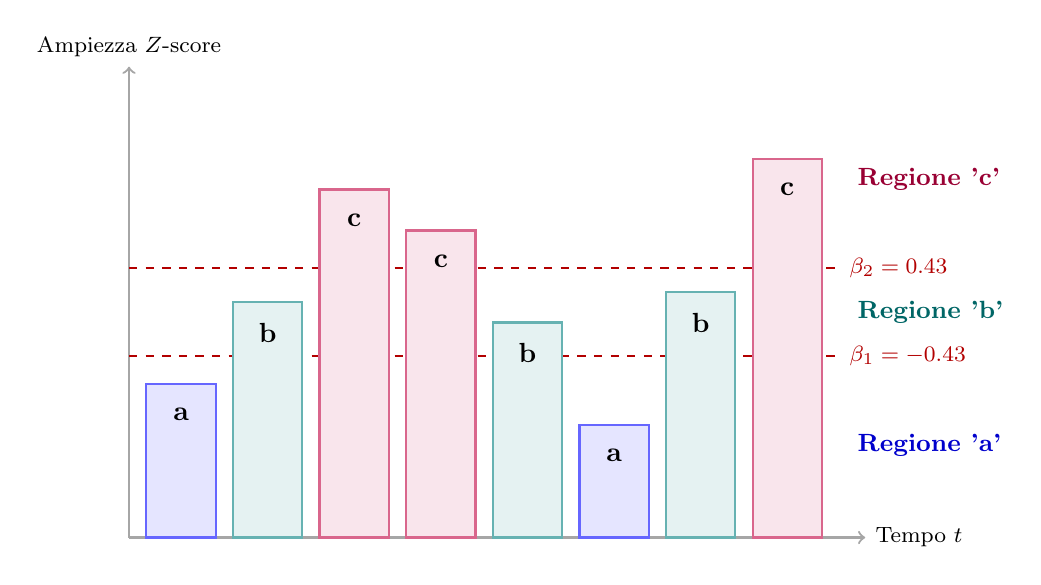
\begin{tikzpicture}[xscale=1.1, yscale=1.3]
    % Assi
    \draw[->, thick, color=gray!70] (0, -2.2) -- (8.5, -2.2) node[right, black] {\footnotesize Tempo $t$};
    \draw[->, thick, color=gray!70] (0, -2.2) -- (0, 2.4) node[above, black] {\footnotesize Ampiezza $Z$-score};

    % Breakpoints e linee orizzontali
    \draw[dashed, red!70!black, thick] (0, 0.43) -- (8.2, 0.43) node[right, red!70!black] {\footnotesize $\beta_2 = 0.43$};
    \draw[dashed, red!70!black, thick] (0, -0.43) -- (8.2, -0.43) node[right, red!70!black] {\footnotesize $\beta_1 = -0.43$};

    % Regioni alfabetiche
    \node[anchor=west, font=\bfseries\small, text=purple!80!black] at (8.3, 1.3) {Regione 'c'};
    \node[anchor=west, font=\bfseries\small, text=teal!80!black] at (8.3, 0.0) {Regione 'b'};
    \node[anchor=west, font=\bfseries\small, text=blue!80!black] at (8.3, -1.3) {Regione 'a'};

    % Blocchi PAA (8 finestre)
    \draw[fill=blue!10, draw=blue!60, thick] (0.2, -2.2) rectangle (1.0, -0.7);
    \draw[fill=teal!10, draw=teal!60, thick] (1.2, -2.2) rectangle (2.0, 0.1);
    \draw[fill=purple!10, draw=purple!60, thick] (2.2, -2.2) rectangle (3.0, 1.2);
    \draw[fill=purple!10, draw=purple!60, thick] (3.2, -2.2) rectangle (4.0, 0.8);
    \draw[fill=teal!10, draw=teal!60, thick] (4.2, -2.2) rectangle (5.0, -0.1);
    \draw[fill=blue!10, draw=blue!60, thick] (5.2, -2.2) rectangle (6.0, -1.1);
    \draw[fill=teal!10, draw=teal!60, thick] (6.2, -2.2) rectangle (7.0, 0.2);
    \draw[fill=purple!10, draw=purple!60, thick] (7.2, -2.2) rectangle (8.0, 1.5);

    % Simboli assegnati
    \node[font=\bfseries] at (0.6, -1.0) {a};
    \node[font=\bfseries] at (1.6, -0.2) {b};
    \node[font=\bfseries] at (2.6, 0.9) {c};
    \node[font=\bfseries] at (3.6, 0.5) {c};
    \node[font=\bfseries] at (4.6, -0.4) {b};
    \node[font=\bfseries] at (5.6, -1.4) {a};
    \node[font=\bfseries] at (6.6, -0.1) {b};
    \node[font=\bfseries] at (7.6, 1.2) {c};
\end{tikzpicture}%
}
\caption{Discretizzazione SAX con alfabeto ternario $\{a, b, c\}$ su $w=8$ finestre PAA. La parola risultante \`e \texttt{abccbabc}.}
\label{fig:sax-discretization}
\end{figure}

\FloatBarrier
\subsection{Criteri di Selezione della Metrica di Similarit\`a}
\label{subsec:ts-metric-selection-guidelines}

La scelta ottimale della misura di distanza dipende dalle dimensioni e dalla natura intrinseca del segnale:
\begin{itemize}
    \item \textbf{Serie Temporali Brevi ($n \le 10^3$)}: si adotta preferenzialmente il \textbf{Dynamic Time Warping (DTW)}, calibrando la dimensione della finestra di warping $r$ per via sperimentale (prevenendo derive patologiche ed accelerando l'elaborazione).
    \item \textbf{Serie Temporali Lunghe ($n > 10^3$)}:
    \begin{itemize}
        \item In presenza di \textbf{conoscenza di dominio}: si estraggono vettori di feature statistiche, dinamiche e spettrali (\textit{feature engineering}), applicando metriche euclidee o modelli supervisionati nello spazio compatto $\R^d$.
        \item In assenza di \textbf{conoscenza a priori}: si impiegano misure non parametriche universali basate sulla compressione e sull'approssimazione simbolica, quali il \textbf{CDM} o \textbf{SAX}.
    \end{itemize}
\end{itemize}

% ====================================================================
% SEZIONE 14.8: CLUSTERING DI SERIE TEMPORALI
% ====================================================================
\FloatBarrier
\section{Clustering di Serie Temporali}
\label{sec:ts-clustering}

Il clustering per serie temporali estende il paradigma dell'apprendimento non supervisionato alle sequenze continue, raggruppando le traiettorie in partizioni omogenee tali da massimizzare la coesione interna e la separazione reciproca inter-cluster.

\FloatBarrier
\subsection{Tassonomia del Clustering per Sequenze Temporali}
\label{subsec:ts-clustering-taxonomy}

Si distinguono quattro configurazioni metodologiche fondamentali:
\begin{enumerate}
    \item \textbf{Whole Clustering}: partiziona un archivio discreto composto da serie temporali indipendenti, assegnando l'intera traiettoria di ciascuna sequenza a un cluster (analogo al partizionamento di record tradizionali in $\R^d$).
    \item \textbf{Feature-Based Clustering}: esegue preventivamente l'estrazione di feature o motivi frequenti (\textit{motifs}) da ciascuna sequenza, applicando algoritmi standard (K-Means, DBSCAN) sullo spazio euclideo dei descrittori.
    \item \textbf{Compression-Based Clustering}: comprime le sequenze convertite in formato simbolico e applica matrici di dissimilarit\`a derivate da misure di complessit\`a dell'informazione (come il CDM).
    \item \textbf{Subsequence Clustering}: opera su una singola serie temporale continua estesa, estraendo sotto-sequenze parziali sovrapposte mediante lo scorrimento di una finestra mobile (\textit{sliding window}) ed aggregando tali segmenti in pattern ricorrenti.
\end{enumerate}

\FloatBarrier
\subsection{Clustering Gerarchico (Hierarchical Clustering)}
\label{subsec:ts-hierarchical-clustering}

Il clustering gerarchico agglomerativo (\textit{bottom-up}) costruisce un albero tassonomico (dendrogramma) senza richiedere la pre-specificazione a priori del numero di raggruppamenti $K$:
\begin{enumerate}
    \item Si calcola la matrice simmetrica delle distanze a coppie tra le $N$ serie temporali impiegando DTW o la metrica Euclidea opportunamente normalizzata.
    \item Si inizializza ogni serie come un cluster singleton disgiunto.
    \item Si aggregano iterativamente i due cluster a minima distanza secondo un criterio di collegamento prefissato (\textit{Single Linkage}, \textit{Complete Linkage}, \textit{Average Linkage} o \textit{Metodo di Ward}).
\end{enumerate}
\textbf{Complessit\`a Computazionale}: La costruzione della matrice delle distanze su $N$ serie di lunghezza $n$ con DTW richiede tempo $\BigO{N^2 \cdot n^2}$ e memoria $\BigO{N^2}$, scalando difficilmente oltre poche centinaia di sequenze.

\FloatBarrier
\subsection{Clustering Partizionale: K-Means per Serie Temporali}
\label{subsec:ts-partitional-kmeans}

Il clustering partizionale suddivide l'insieme delle sequenze in $K$ gruppi esaustivi e disgiunti minimizzando la devianza intra-cluster (\textit{Sum of Squared intra-cluster Errors}, SSE):
\begin{equation}
\label{eq:ts-kmeans-sse}
\mathrm{SSE} = \sum_{k=1}^K \sum_{X_i \in C_k} D(X_i, \boldsymbol{\mu}_k)^2
\end{equation}
dove $\boldsymbol{\mu}_k$ rappresenta il profilo medio o centroide del cluster $C_k$, e $D$ \`e la metrica di distanza prescelta.

\begin{itemize}
    \item \textbf{Centroide Euclideo}: Sotto distanza Euclidea, il centroide \`e calcolato banalmente dalla media aritmetica punto per punto delle serie appartenenti al cluster:
    \begin{equation}
    \boldsymbol{\mu}_k(t) = \frac{1}{|C_k|} \sum_{X_i \in C_k} X_i(t)
    \end{equation}
    \item \textbf{Centroide sotto DTW (DTW Barycenter Averaging - DBA)}: Sotto DTW, la media aritmetica punto per punto \`e priva di significato fisico a causa degli sfasamenti temporali. Il centroide deve essere ricavato mediante algoritmi di allineamento multiplo elastico (\textit{DBA}), che mediano le coordinate connesse lungo i rispettivi warping path.
    \item \textbf{Vulnerabilit\`a}: Richiede di fissare $K$ a priori ed \`e sensibile alla scelta dell'inizializzazione dei centroidi e alla presenza di outlier isolati.
\end{itemize}
